\chapter{Additional methodological details, data, and \\site
	descriptions}\label{dx:C}
\chaptermark{Additional methods and site descriptions}

This section provides additional, unpublished information regarding
methods or field observations that support the research presented in
the preceding chapters.

\section{\texorpdfstring{Equilibrium 
		Δ\textsuperscript{13}CH\textsubscript{3}D versus
		temperature}{Calculated equilibrium Δ13CH3D versus temperature}}\label{calculated-equilibrium-ux3b413ch3d-versus-temperature}

\mrefs[B]{Figure}{fig:C:2} shows the calculated values of ln \emph{K}\textsubscript{eq} vs.\ temperature for the reaction:
\begin{equation}\label{eqn:C:exchange}
{}^{13}\text{CH}_4+ {}^{12}{\text{CH}}_3\text{D}\rightleftharpoons {}^{13}{\text{CH}}_3\text{D}+ {}^{12}{\text{CH}}_4 
\end{equation}

\noindent A good fit to the curve is obtained with the expression:
\begin{equation}\label{eqn:C:equilibrium}
1000\ln K = \left( 1.68169 \times 10^{14} \right)\left( \frac{1}{T^{2}} \right)^{3} - \left( 1.40754 \times 10^{10} \right)\left( \frac{1}{T^{2}} \right)^{2} + \left( 6.72697 \times 10^{5} \right)\left( \frac{1}{T^{2}} \right) - 0.28671
\end{equation}
where temperature \emph{T} is in kelvin.


\begin{figure*}
	\centering
	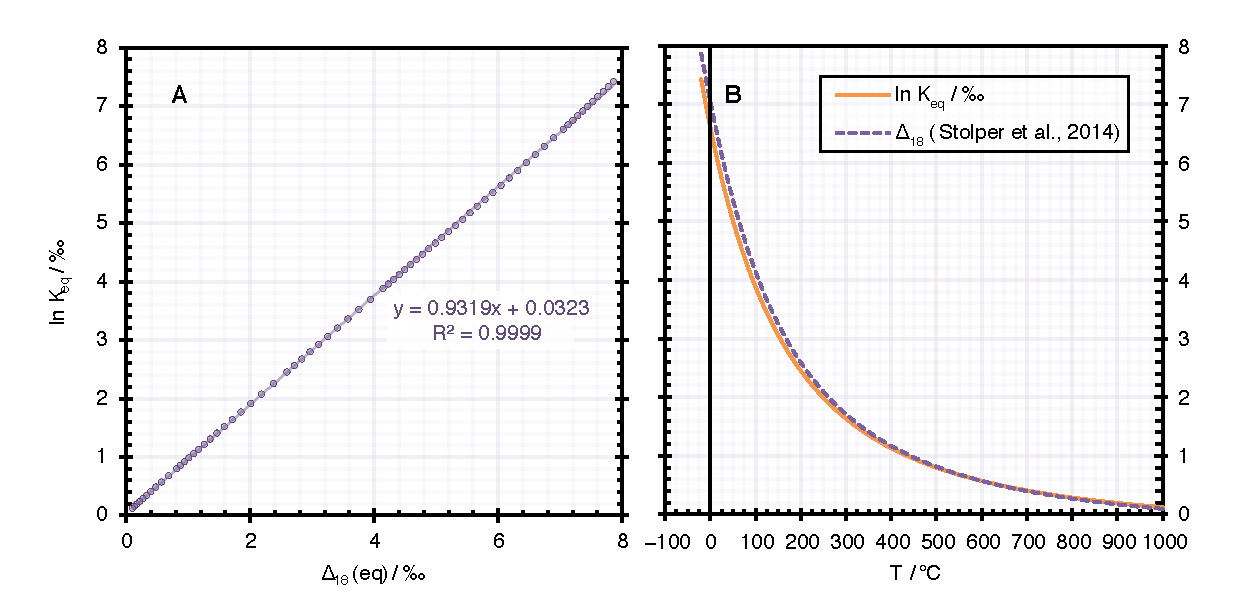
\includegraphics[width=\textwidth]{figures/FigC.2}
	\captionsetup{format=myformat}	% hrule beneath caption
	\caption[Equilibrium Δ\textsubscript{18} and Δ\textsuperscript{13}CH\textsubscript{3}D values as a function of temperature]{Equilibrium Δ vs.\ $T$ curves.  (\textbf{A}) Conversion between equilibrium
		Δ\textsubscript{18} values and equilibrium
		Δ\textsuperscript{13}CH\textsubscript{3}D values. Note that conversion
		of Δ\textsubscript{18} to Δ\textsuperscript{13}CH\textsubscript{3}D can
		only be done if it is known or can be assumed that methane isotopologues
		have attained their equilibrium distribution at the temperature
		indicated by both Δ\textsuperscript{13}CH\textsubscript{3}D and Δ\textsuperscript{12}CH\textsubscript{2}D\textsubscript{2}. Nonequilibrium
		Δ\textsubscript{18} values cannot easily be converted to
		Δ\textsuperscript{13}CH\textsubscript{3}D, particularly if Δ \textless{}
		0 ‰ (anticlumped). (\textbf{B}) Comparison between equilibrium
		Δ\textsuperscript{13}CH\textsubscript{3}D [= ln
		\emph{K}\textsubscript{eq} for the isotope exchange reaction (\autoref{eqn:C:exchange}), defined
		following \textcite{Ono++_2014_AC} and calculated as in \textcite{Wang++_2015_S}], and equilibrium Δ\textsubscript{18}
		values from \textcite{Stolper++_2014_GCA}.}
	\label{fig:C:2}
\end{figure*}

\section{Notes on analytical procedures}

\subsection{\texorpdfstring{Isolation of CH\textsubscript{4} using
		cryofocusing-preparative gas
		chromatography}{Isolation of CH4 using cryofocusing-preparative gas chromatography}}\label{isolation-of-ch4-using-cryofocusing-preparative-gas-chromatography}

\begin{sidewaysfigure}
%	\centering
	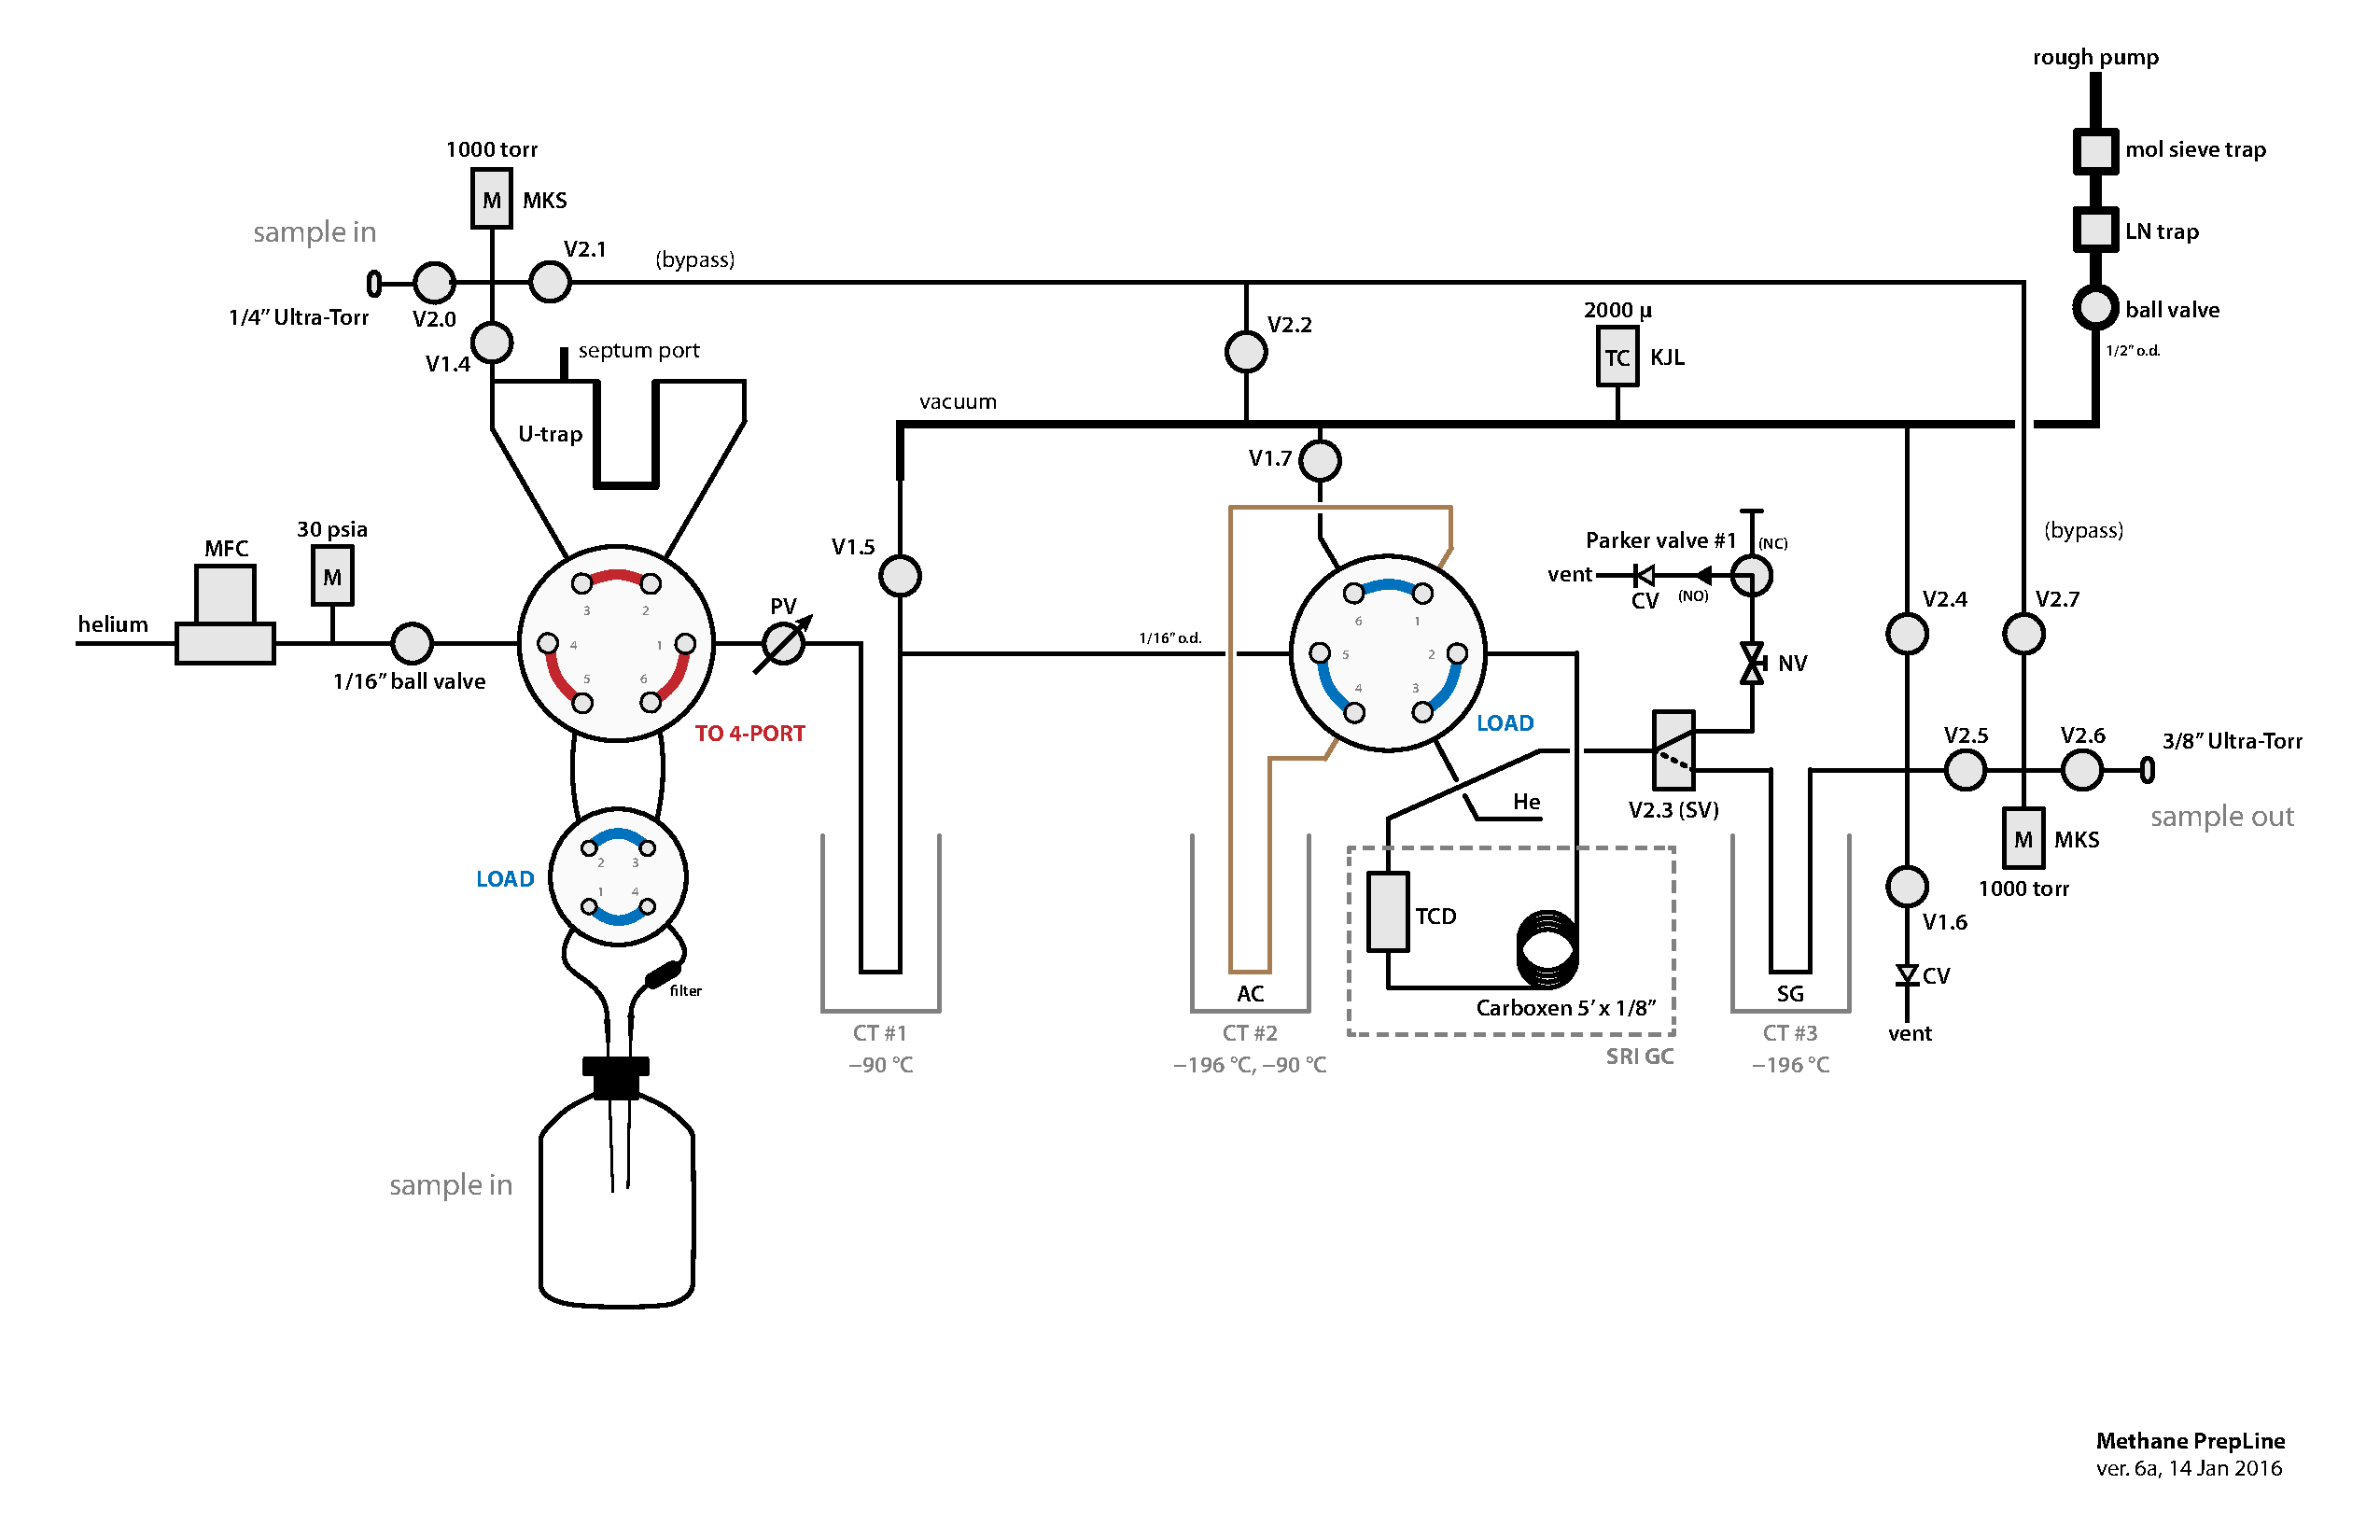
\includegraphics[width=\textwidth]{figures/FigC.1.pdf}
	\caption[Schematic of methane preparation system]{Schematic of methane preparation system at the MIT
		Hardcore Stable Isotope Laboratory.}
	\label{fig:C:1}
\end{sidewaysfigure}


\mrefs[]{Figure}{fig:C:1} shows a schematic of the methane preparation system used to
isolate CH\textsubscript{4} for measurement of
Δ\textsuperscript{13}CH\textsubscript{3}D by TILDAS at MIT from mid-2014
onwards \parencite{Wang++_2015_S,Inagaki++_2015_S,Wang++_2016_GCA,Lopes++_2016_JoDS,Whitehill++_2017_GCA}. The system consists of a
cryotrapping-preparative gas chromatography system interfaced with a
vacuum line and a helium supply. A software interface built using
National Instruments LabVIEW controls all pneumatically- and
electronically-actuated valves, pistons for dewars on cold traps, and
heating coils. Operation is mostly automatic and hands-free.
Preparation time is \textless{}45~minutes for a typical sample of
1--15~cm\textsuperscript{3} SATP CH\textsubscript{4} and
\textless{}200~cm\textsuperscript{3} air. Air blanks in the purified gas
are typically \textless{}0.10~cm\textsuperscript{3} SATP.

The retention time of methane on the PrepLine column depends on the amounts of both \ce{CH4} and ``air'' (\ce{O2}, \ce{Ar}, \ce{N2}, \ce{CO})
in the sample, as shown in \autoref{fig:C:GC}.

\begin{SCfigure*}
	\centering
	\includegraphics[width=0.55\linewidth]{figures/FigC.GC}
	\caption[Dependence of the retention time of \ce{CH4} on volumes of \ce{CH4} and air on the PrepLine]{Dependence of the retention time of \ce{CH4} (\emph{x}-axis) on on-column volumes of \ce{CH4} (\emph{y}-axis) and ``air'' (= \ce{O2} + Ar + \ce{N2} + \ce{CO}) on the Prep\-Line.  The sample is heated off cold trap \#2 and injected onto the column between 15~seconds and 1~minute.  Compounds in order of elution are \ce{H2}, air, \ce{CH4}, and \ce{CO2} + \ce{C_{2+}}.}
	\label{fig:C:GC}
\end{SCfigure*}

\subsection{Correction of non-linearity in isotopologue concentration
	data}\label{correction-of-non-linearity-in-isotopologue-concentration-data-returned-by-tdlwintel}

Data retrieved from TDLWintel (Aerodyne Research, Inc., Billerica, Mass.)\footnote{For a history of the development of TDLWintel for applications with tunable diode and quantum cascade laser instruments, see \textcite{Horii++_1999_SPIE,Zahniser++_1995_PTRSA,Nelson++_2002_ApplPhysB,Nelson++_2004_SA-A}.} are in the form of number
densities (ND) that the software calculates from line parameters in the HITRAN database \parencite{Brown++_2013_JQSRT,Rothman++_2013_JQSRT}. For
all clumped isotopologue data collected in this thesis except those in
\autoref{dx:A}, the following correction scheme was applied.  Isotopologue/isotope ratios reported were calculated from the corrected number densities ($\mathrm{ND}_{6x}^\mathrm{corr}$).  
\begin{equation}\label{eqn:C:correction}
\mathrm{ND}_{6x}^\mathrm{corr} = \mathrm{ND}_{6x}^\mathrm{meas} + D_{6x} \cdot \mathrm{ND}_{61}^\mathrm{meas} + H_{6x} \cdot \mathrm{ND}_{61}^\mathrm{meas} \cdot \left(1 - \frac{\mathrm{ND}_{61}^\mathrm{meas}/P_\mathrm{meas}}{\mathrm{ND}_{61}^\mathrm{pure}/P_\mathrm{target}} \right)~
\end{equation}
Here, $\mathrm{ND}_{6x}^\mathrm{meas}$ are the number densities returned by TDLWintel in the \texttt{STR} files, $P_\mathrm{meas}$ is the pressure of the sample in the cell, $P_\mathrm{target}}$ = \SI{1.0383}{\torr}, and $\mathrm{ND}_{61}^\mathrm{pure}$ (= \num{3.88e6}) is the number density of \ce{^{12}CH4} for a sample of pure methane at the target pressure.  
Calibrated values for the correction factors $D$ and $H$ are listed in \autoref{tab:C:correctionfactors}.  Note that the $D$ and $H$ here are just variable names, and are not related to deuterium or hydrogen.  Numbering of isotopologues is from HITRAN.
\begin{SCtable*}[][bp]
	\centering
	\caption[Correction factors applied to measured number densities]{Correction factors for \autoref{eqn:C:correction}. Values were determined during 2014--2015.  Values for $D$ were derived from measurements of methane heated to equilibrium over a catalyst, and values for $H$ were derived from measurements of methane admixed with different percentages of \ce{N2} in the TILDAS cell.}
	\label{tab:C:correctionfactors}
	\begin{tabular}{clcd{4}}
	\toprule
	\# & isotopologue & $D$ & H\tabularnewline
	\midrule
	61 & \textsuperscript{12}CH\textsubscript{4} & 0 & 0\tabularnewline
	62 & \textsuperscript{13}CH\textsubscript{4} & 0 & -0.0033\tabularnewline
	63 & \textsuperscript{12}CH\textsubscript{3}D & 0 & -0.0036\tabularnewline
	64 & \textsuperscript{13}CH\textsubscript{3}D & \num{3.00e-3} & -0.0125\tabularnewline
	\bottomrule
	\end{tabular}
\end{SCtable*}

I have found this correction scheme to sufficiently correct the observed
non-linearity in δ\textsuperscript{13}CH\textsubscript{3}D vs.\ δ\textsuperscript{12}CH\textsubscript{3}D over a wide range of
δ\textsuperscript{12}CH\textsubscript{3}D values (from $-$600 to +400‰ vs.\ AL1) (the $D$ term), as well as any air that might make its way into the system (up to
10\%) (the $H$ term; the portion enclosed in parentheses represents an estimate of the percentage impurity in the methane sample).\footnote{The $D$ term 
corrects the observation that measured Δ\textsuperscript{13}CH\textsubscript{3}D values are lower than their true values when δD of the sample 
is lower than that of the reference gas (and vice versa).  The $H$ terms correct an observed elevation in all three δ-values when impurities (primarily air) are 
present in the sample (important for the recycling technique used on small samples because air can accumulate in the sample due to small leaks in the TILDAS inlet system).}
Part of the reason for the nonlinearity is that the Voigt profile cannot accurately account for the tailing of one or more large \textsuperscript{12}CH\textsubscript{4} peaks
that are located immediately outside the wavelength region scanned by the laser.

\subsection{Calibration of isotopic composition of in-house standards
	(AL1)}\label{calibration-of-isotopic-composition-of-in-house-standards-al1}

%\input{tables/tableC.2}

The δ\textsuperscript{13}C and δD values we report have been calibrated
relative to PDB and SMOW, respectively, by measuring samples of NGS-1
(also known as NIST SRM 8559 and USGS-A) and NGS-3 (also known as NIST
SRM 8561 and USGS-C), which are natural gas standards with published
reference values for δ\textsuperscript{13}C and δD, as listed in \autoref{reporting-of-ux3b413c-and-ux3b4d-values} \parencite[supplementary materials in][]{Wang++_2015_S}. Samples of these natural gases were
included in a set of calibration samples distributed by the USGS to
various laboratories in the U.S. in July 2014. These samples were
contained in IsoTubes (Isotech Laboratories, Illinois, USA) at pressures
of \textasciitilde{}3 bar. We subsampled aliquots of these gases through
a septum adapter fitting (available from Isotech) using a 25~ml gastight
syringe (SGE Analytical Science), and introduced the aliquots into our
sample preparation system as described above.

Data shown in this thesis for δ\textsuperscript{13}C, δD, and
Δ\textsuperscript{13}CH\textsubscript{3}D assume that reference gas AL1
has the isotopic composition $-$34.5‰, $-$147.7‰, and $+$2.41 ± 0.07‰ (95\% CI)
respectively, consistent with \textcite{Wang++_2015_S} and with the values we
provided to the UCLA group \parencite{Young++_2016_IJMS}.\footnote{The values originally reported in \textcite{Ono++_2014_AC} are quite different in δD (by \textasciitilde{}20‰) for reasons as yet undetermined.  Anecdotal experience suggests that this is probably related to a historical problem of poorly-anchored δD values for GC-IRMS analyses of methane within the isotope community, with resultant differences in calibration between the several IRMS labs from which values for δD
of AL1 vs.\ SMOW were obtained.  I favor the revised values listed above for reasons of consistency with the NGS gases and the new USGS samples.} 

\section{Miscellaneous unpublished information on selected sites}\label{miscellaneous-unpublished-information}

This section contains miscellaneous data and ruminations that do not yet have a proper home in the literature.
\clearpage 

\subsection{\texorpdfstring{Additional field notes and thoughts on selected localities studied by \textcite{Wang++_2015_S}}{Additional field notes and thoughts on selected localities studied by Wang et al.\ (2015)}}\label{field-notes-and-thoughts-on-selected-localities}

\subsubsection{Lower Mystic Lake}\label{lower-mystic-lake}

The water sample from Lower Mystic Lake shown in \autoref{ch:2} was sampled from the water column at a depth of 18 mbll,
which is below the chemocline. It should be noted that the isotopic
composition of pore waters in Lower Mystic Lake sediments, at the
time(s) and depth(s) at which the methane was generated, may be or have
been significantly different than that of the water in the water column.
This is because prior to the implementation of water management
practices, Lower Mystic Lake was tidally-influenced, and the bottom waters were derived from seawater that flowed upriver along the bottom of the Mystic
River. Dams constructed in 1908 and 1966 slowed or stopped the influx of
seawater, and initiated a gradual reduction in the volume of anoxic and
sulfidic bottom waters in the lake; the reduction in bottom waters was
also accelerated by intentional removal of bottom waters by pumping and
treatment in the 1980s and 1990s \parencite{Duval+Ludlam_2001_IRHb,Ludlam+Duval_2001_LRM}. Therefore, even though the δD of Lower Mystic Lake water
at 18 mbll ($-$40.6 ± 1.0‰, 1\emph{s}) was similar to that of Upper Mystic
Lake ($-$39.2 ± 1.8‰, 1\emph{s}), the Lower Mystic Lake sediment pore
waters may have an isotopic signature that is closer to that of seawater
(\textasciitilde{}0‰). This trend is observed in other coastal
meromictic lakes in which seawater is trapped below the chemocline
\parencite{Jeffries++_1984_CJES}. Assuming a value of 0‰ for the associated
waters for methane generated in Lower Mystic Lake sediments would not
affect our conclusions; on the contrary, it would suggest that the field
of primary microbial methane could be constrained even more tightly than
\autoref{fig:2:2} indicates.

\subsubsection{CROMO}\label{cromo}

The water sample from the Coast Range Ophiolite Microbial Observatory (CROMO) for which the δD\textsubscript{water} value
is reported in \autoref{ch:2} was collected from the CSWold well. This well
is noted in publicly-available reports on water quality monitoring in
the area, but we do not presently have information on the depth(s) at
which the groundwater at CSWold is derived. However, the δD value of the
water is consistent with mixing between deep sedimentary-derived brines
and meteoric waters \parencite{Peters_1993_GCA}.

At CROMO, the δ\textsuperscript{13}C and δD data alone cannot
conclusively distinguish between thermogenic, abiogenic, and microbial
origins of the methane. Specifically, the CROMO gases are highly similar
in δ\textsuperscript{13}C and δD to the sample of natural gas from the
Utica Shale (\autoref{tab:2:S1} and \autoref{fig:2:1}), where the gases are
generally inferred to have been generated by thermogenic processes. The
Δ\textsuperscript{13}CH\textsubscript{3}D values at each field site are
very dissimilar, however, with the Utica Fm. gases having an apparent
temperature \textasciitilde{}160~°C and the CROMO gases having apparent
temperatures of 42 to 76~°C. Therefore, the clumped isotopic measurement
provides information that is complementary to, and independent of, the
bulk δ\textsuperscript{13}C and δD data, a conclusion that is not
obvious from previous studies.

I suggest that at CROMO, the isotopic composition of the gases
(δ\textsuperscript{13}C, δD, and
Δ\textsuperscript{13}CH\textsubscript{3}D) is inconsistent with a
significant contribution from thermogenic sources of methane.\footnote{Note that this is somewhat different from what was written by \textcite{Wang++_2015_S}.}
Furthermore, the C\textsubscript{1}/C\textsubscript{2} ratio (measured
using GC-FID) ranged from 360 to 1540 (\autoref{tab:2:S5}) for
samples of dissolved gases collected from 5 wells (including N-, CSW-,
and QV- wells) sampled in July 2014; these
C\textsubscript{1}/C\textsubscript{2} ratios are within the range
expected for microbial gases (\textgreater{}100), and outside the range
of values typically observed for thermogenic gases (\textless{}100).

If the framework presented in \autoref{fig:2:2} is correct, then a major source of
uncertainty in differentiating between the possible processes of methane
generation is the δD of the associated waters from which methane was
produced. Specifically, meteoric water in the vicinity of CROMO
generally has lower δD values ($-$70 to $-$50‰) \parencite{Peters_1993_GCA,Kendall+Coplen_2001_HP} than what was measured for water from the CSWold well
($-$33‰; \autoref{tab:2:S5}). Previous work on natural springs in the
vicinity of the McLaughlin mine suggested that groundwater in this
region can be best characterized as a two-component mixture consisting
of formation brines derived from the Great Valley Sequence mixed with
variable amounts of low-salinity meteoric water \parencite{Peters_1993_GCA}.
Parenthetically, I note that the
Δ\textsuperscript{13}CH\textsubscript{3}D-based temperatures for methane
at CROMO (42 to 76~°C) would suggest isotopic equilibration with water
that has a δD in the range of 0 to +20‰ (\autoref{fig:2:2}). This range is
consistent with the δD value (+11‰) of the most saline waters
({[}Cl\textsuperscript{\textminus}{]} \textasciitilde{} 580 mmol/kg) sampled by
\textcite{Peters_1993_GCA} from springs in the vicinity of CROMO. The apparent
temperatures of 42 to 76~°C for methane at CROMO are within the accepted
temperature limits of life (generally \textless{}80~°C, but up to 122~°C
for hyperthermophilic methanogens). Thus, based on the consistency of
the observed isotopic signatures with other geochemical parameters
(namely, {[}H\textsubscript{2}{]}, \autoref{fig:2:3}), I infer a
dominantly-microbial origin of the methane at CROMO originating from deep groundwater below the ophiolite body. Methanogenesis does not appear to occur to any appreciable extent in the shallow (meteoric) groundwaters.  More recent microbiological work showing a total absence of archaea, including methanogens, from 16S sequences of the CROMO waters  \parencite{Twing++_2017_FMicro} appears to support this conclusion.   

\subsection{Methane isotopologue data on assorted samples}

\begin{table}\centering
	
	\caption[Isotopologue data for assorted methane samples]{Isotopologue data for methane samples from a rice paddy in Sherrill, Arkansas, USA, and the Chimaera seepage, Tekirova ophiolite, Turkey. Uncertainties
		reported are 95\% confidence intervals. Values for
		δ\textsuperscript{13}C, δD, and
		Δ\textsuperscript{13}CH\textsubscript{3}D are reported relative to PDB,
		SMOW, and the stochastic distribution, respectively.}
	\label{tab:C:3}

	\begin{threeparttable}
		
		\begin{tabular}{@{} l l r@{\hspace{0.2em}}l r@{\hspace{0.2em}}l >{\raggedleft\arraybackslash}p{2.5em}@{\hspace{0.2em}}l r@{\hspace{0.2em}}l @{}}
			% This notation >{\raggedleft\arraybackslash}p{5em} is for padding the left side so that multicolumn doesn't expand extra space on the right column of the multicolumn{2}{c}. http://stackoverflow.com/a/25690685
			\toprule
			Site & Sample Name & \multicolumn{2}{c}{δ\textsuperscript{13}C (‰)} & \multicolumn{2}{c}{δD (‰)} &
			\multicolumn{2}{c}{Δ\textsuperscript{13}CH\textsubscript{3}D (‰)} & \multicolumn{2}{c}{\textit{T}\textsubscript{13D}
				(°C)}\tabularnewline
			\midrule
			Sherrill & JTB-1-2 & \textbf{$-$56.40} & ± 0.05  & \textbf{$-$336.47} & ± 0.05  &
			 \textbf{$-$0.47} & ± 0.23  & \textbf{a.c.} &  \tabularnewline
%			\midrule
			Chimaera* & S8\_271949\_4034797\_12.10.2013 & \textbf{$-$11.41} & ± 0.03  & \textbf{$-$119.50} & ± 0.05  &
			\textbf{3.19} & ± 0.18  & \textbf{141} & +13/$-$12 \tabularnewline
			& S4 & \textbf{$-$11.62} & ± 0.10  & \textbf{$-$119.57} & ± 0.10  &
			\textbf{2.62} & ± 0.54  & \textbf{185} & +55/$-$42 \tabularnewline
			& S5 & \textbf{$-$11.37} & ± 0.10  & \textbf{$-$119.42} & ± 0.10  &
			\textbf{2.98} & ± 0.43  & \textbf{156} & +35/$-$29 \tabularnewline
			& S9 & \textbf{$-$11.38} & ± 0.12  & \textbf{$-$119.49} & ± 0.14  &
			\textbf{3.32} & ± 0.34  & \textbf{133} & +23/$-$21 \tabularnewline
			\bottomrule
		\end{tabular}
	
		\begin{tablenotes}
			\item * Samples from Chimaera were measured more than 6 months apart (May to December 2014).  The data appear to be unaffected by storage or instrumental drift over this period.
		\end{tablenotes}
	
	\end{threeparttable}
\end{table}




\subsubsection{Rice paddy, Sherrill, Arkansas, USA}\label{rice-paddy}
A sample of gas was collected by J.T. Bird from a paddy rice field in Sherrill, Arkansas, USA in June of 2014.  Bubbles of gas were released by gentle agitation of the submerged sediment, trapped in a funnel, and transferred to serum bottles containing several milliliters of 1~M NaOH added to inhibit microbial activity.  On the day of collection, air temperature was 93~°F and skies were cloudy.  Given that the daily lows had been steady at 70~°F for five days and the water on the field had been standing for ``a good two weeks'' (Sherrill local, via J.T. Bird, pers.\ comm.), estimated water temperatures are \textasciitilde{}75~°F or about 25~°C.  

Analysis of methane in the sample (\autoref{tab:C:3}) yielded relatively low δ\textsuperscript{13}C and δD values ($-$56‰ and $-$336‰) typical of biologically-produced methane in wetlands.  The Δ\textsuperscript{13}CH\textsubscript{3}D value was anticlumped (ca.\ $-$0.5‰).  This is the lowest degree of \textsuperscript{13}C--D clumping we have observed in any natural methane sample aside from seep gases at The Cedars.  

\subsubsection{Chimaera seep, Tekirova ophiolite, Turkey}
Four samples of gases collected by H.\ Hoşgörmez from the Chimaera seep (Yanartaş, meaning ``flaming rock'', near the Gulf of Antalya, eastern Mediterranean Sea; also the source of the first Olympic flame)   were sent to us by G.\ Etiope.  Samples arrived in glass vessels equipped with gas-tight stopcocks at both ends.  

Analyses of methane in these samples yielded relatively high bulk δ\textsuperscript{13}C and δD values ($-$11‰ and $-$119‰, \autoref{tab:C:3}) consistent with those previously reported for the same site \parencite{Etiope++_2011_EPSL,Hosgormez++_2008_Gf,Hosgormez_2007_JAsES}.  The δ\textsuperscript{13}C values lie outside the typical range of known thermogenic methane (up to $-$20‰), and δD values are close to those required for D/H equilibrium with water of SMOW-like hydrogen-isotope composition at temperatures upwards of ca.\ 200~°C (\autoref{fig:3:5}).  The Δ\textsuperscript{13}CH\textsubscript{3}D data indicated apparent equilibrium temperatures averaging 153~°C.  These temperatures are much higher than the \textless50~°C temperatures at which abiotic methane was inferred by \textcite{Etiope++_2011_EPSL} to be synthesized here.  Recently-published data obtained by the UCLA group on several other samples taken at Chimaera yielded Δ\textsuperscript{13}CH\textsubscript{3}D values (ranging from +3.3 to +3.6‰) in general agreement with ours, as well as Δ\textsuperscript{12}CH\textsubscript{2}D\textsubscript{2} values that are at or near equilibrium at the same temperatures indicated by Δ\textsuperscript{13}CH\textsubscript{3}D \parencite{Young++_2017_GCA}.  These data indicate that methane carrying clumped isotopologue abundances similar to those of typical thermogenic gases probably comprises a large fraction of the Chimaera seep gas and that such gases may contribute more to the seepage flux than was previously suggested.  



\section{Errata and corrigenda to published articles} \label{errata}

The following mistakes have been found in the two articles published from this thesis.
\begin{description}
	\item[\textcite{Wang++_2015_S}]  (\emph{i}) In Figure S4, the arrows denoting secondary isotope fractionation were labeled incorrectly; this is corrected in \autoref{fig:2:S4}.  (\emph{ii}) Several footnotes in Table S3 were incomplete or incorrectly labeled; this is fixed in \autoref{tab:2:S3}.  (\emph{iii}) Samples from the Powder River Basin were misstated as being from Wyoming.  These samples were actually taken from wellheads located in Montana, near the border with Wyoming (API well numbers 25-003-22076, 25-003-22192, and 25-003-22074, in order of appearance in \autoref{tab:2:S1}).  Also, well ``3CA34'' was completed in the Cook Coal as stated in the paper, but produces from the stratigraphically-higher Canyon Coal according to information on the Montana Board of Oil \& Gas Conservation website. \autoref{ch:2} contains the corrected information.  Several typographical errors have also been corrected.
	\item[\textcite{Wang++_2016_GCA}]  In Table 2, citations to the \citeauthor{Joelsson++_2014_CPL} papers were inadvertently switched.  \textcite{Joelsson++_2015_ACPD,Joelsson++_2016_ACP} should be cited for \ce{CH4}~+~OH and \textcite{Joelsson++_2014_CPL} for \ce{CH4}~+~Cl\@.  \autoref{tab:4:2} lists the correct references.
\end{description}



\section{Acknowledgments}
% \addcontentsline{toc}{section}{Acknowledgments}

Shuhei Ono and Bill Olszewski provided key assistance with the design, 
construction, and troubleshooting of the Methane PrepLine.  Kyle Delwiche and Genming Luo are thanked for their help in the field at Lower Mystic Lake, and for insightful conversations.  Discussions with Matt Schrenk, Billy Brazelton, Katrina Twing, Mike Kubo, and Tori Hoehler helped form my views on the CROMO gases.  Dan Ritter provided the information regarding locations of wells in the Powder River Basin.  Jordan Bird graciously went out of his way to sample the Arkansas rice paddy (and take video footage!).  Giuseppe Etiope is thanked for sending us the samples from the Chimaera seep.





